\chapter{Array Evaluation}
\section{Overview}
As stated in chapter \dots the geometry of a microphone array
has a impact on the performance of beamforming.
The goal is to find a well suited array geometry for the detection and tracking of
Drones.
To achieve this, first some array geometries have been simulated and then
a prototype was built to gather information on how they perform in reality.
Then the real data were compared to the simulated data to
confirm the validity of the simulation.
In the next step the findings of the prototypes and simulations
were used to come up with a final array design.

By analysing the sound of some commercially available drones
a desired frequency range of 500 to 2000 hz was set.
This range includes most of the sound's energy.

The array geometry has some contraints, 
such as the number of microphones and the mechanical feasibilty.
As stated in \ref*{chap:AqqSys} the maximum number of microphones
in an array is 32.

To compare different array geometries, several simulations
were ran for each array.
The simulated data was then ran through the beamforming 
algorithm.
The steering angles are based on a grid with $-180^\circ \leq \phi < 180\circ$ and 
$0^\circ \leq \theta \leq 180^\circ$ with a spacing of $1^\circ$.
For each point in this grid the power over the desired frequency band is calculated.
Displaying the result leads to an image like Figure \ref*{aev:fig:gridEx}.
The visualizations may be misleading depending on the angle.
This is a result from the projection of the semisphere onto a 2-d surface.
\begin{figure}
	\centering
	%    \includegraphics[width=0.25\textwidth]{mesh}
	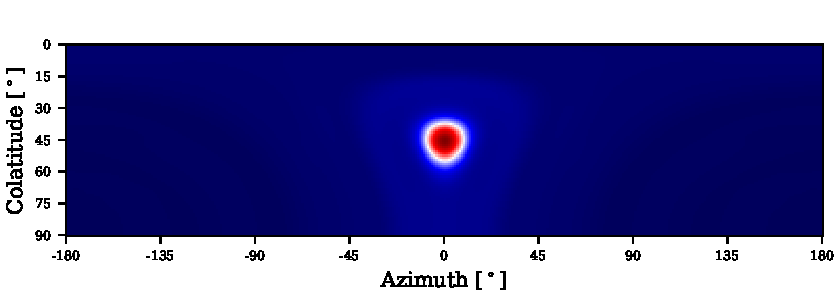
\includegraphics[]{images/5_array_evaluation/0.5_0.79.pdf}
	\caption{PGurke}
	\label{aev:fig:gridEx}
\end{figure}
\section{Metrics}
TO evaluate the performance of an array several metrics are used.
In \todo{Cite Array design s40430-018-1275-5-1, array design comparisons} the
main beam-width is proposed.
\todo{cite Circ array drone trackings13638-019-1632-9} is using the ratio
between the main lobe power and the side lobe power.
Another measure related to the main lobe with is the main lobe area.s
The main lobe is defined as all the points around the peak where their value
is greater than half the peaks value. \todo{besser englisch}

\subsection{Area}
Since the grid resulting from the beamforming represents spherical function
simply taking the sum of all the gridpoints from the mainlobe 
would deliver false results. 
So each grid point is normalized by the surface element of a sphere
\begin{equation}
	dA = r \sin\theta \, d\phi \cdot r d\theta.
\end{equation}
The area of the mainlobe determines how good different sources can be separated.
With a big mainlobe area two close sources may lead to one bigger mainlobe instead
of two seperable ones.
\subsection{Peak Average Power ratio}
The Peak Average Power ratio is the ratio between the peak power and
the average power over the whole grid.
The results from the projection are compenstatet by weighting
the power at each grid cell with the area of that grid cell. 


Blabla
\section{Array Geometry}
In \todo{cite} the authors use a circular array to detect and track drones.
They however did not gave any reasoning no why the chose a circular array.
\cite{bandkProducts}
In \cite{arr1} different array types are compared and measured.
The best scores are reached with the Underbrink style array, a combination
of multiple circular arrays.
They also included several spiral based arrays
Based on this three main groups of arrays were further analysed,
the circualr array, an adaption of the underbrink array, and a archimedes
spiral array.
\subsection{Circular Array}
The circular array is the most simple shape of these three.
It has two degrees of freedom, the circle radius and the number of microphones.
Figure \ref*{aev:fig:MicCirc} shows how the PAP ratio changes when
more microphones are added to an array with a fixed radius.
For smaller array the best PAP they can have is reached with less
microphones than the bigger ones need.
\dots Hallo Satz
The radius of the array has a big impact on how the lower frequencies
smear out the peak.


\begin{figure}
	\centering
	%    \includegraphics[width=0.25\textwidth]{mesh}
	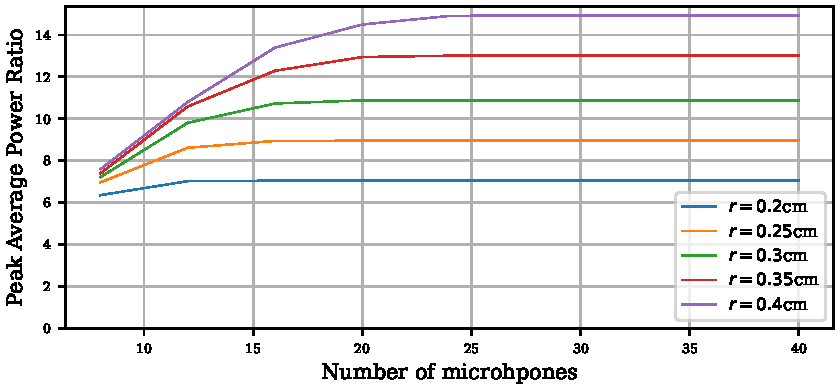
\includegraphics[]{images/5_array_evaluation/circ_m_pap.pdf}
	\caption{PAP ratio for different array radiuses and total number
	of microphones.}
	\label{aev:fig:MicCirc}
\end{figure}
\begin{figure}
	\centering
	%    \includegraphics[width=0.25\textwidth]{mesh}
	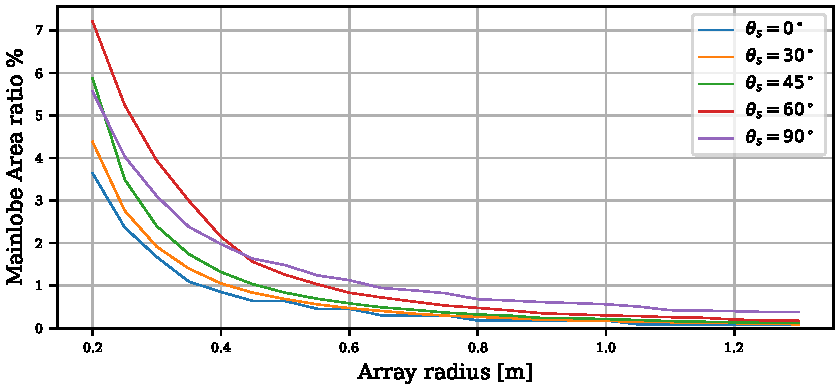
\includegraphics[]{images/5_array_evaluation/area_circ.pdf}
	\caption{Ratio of the mainlobe area compared to the area of a half sphere for 
	a circular array with 32 microphones.}
	\label{aev:fig:areaCirc}
\end{figure}
\begin{figure}
	\centering
	%    \includegraphics[width=0.25\textwidth]{mesh}
	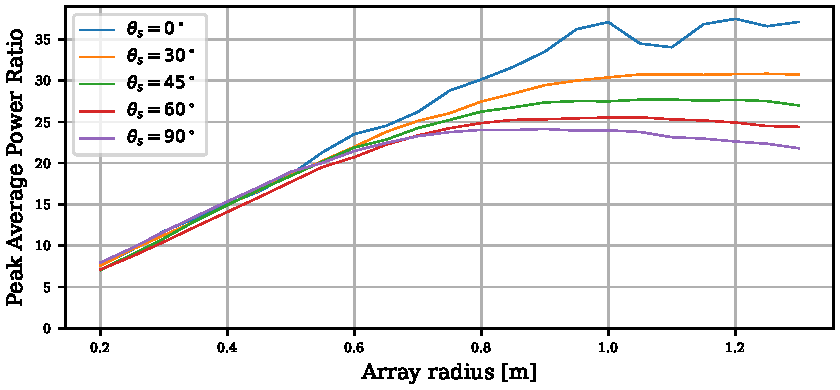
\includegraphics[]{images/5_array_evaluation/PAP_circ.pdf}
	\caption{Peak Average }
	\label{aev:fig:papCirc}
\end{figure}
\dots
\subsection{Underbrink Array}
\dots
\subsection{Archimedes Spiral Array}

\newpage
\section{Mechanical Design}
The mechanical design of the array prototypes was centered around the objective of testing a wide range of array configurations.
To achieve this, two flexible microphone array frames were developed.
A significant aspect of the design process involved determining the overall size of the arrays.
While larger arrays typically offer better performance, practicality and manufacturability had to be considered as well.
In practice, a maximal outer diameter of 60\,cm was chosen for the array prototypes.
Based on simulation results, two specific array types were explored: The Multi-Circular Array and the Archimedean Spiral Array, as described in the next sections.

\subsection{Multi-Circular Array}
\begin{minipage}{\linewidth}
	\begin{wrapfigure}{r}{7.5cm}
		\vspace{-0.8cm}
		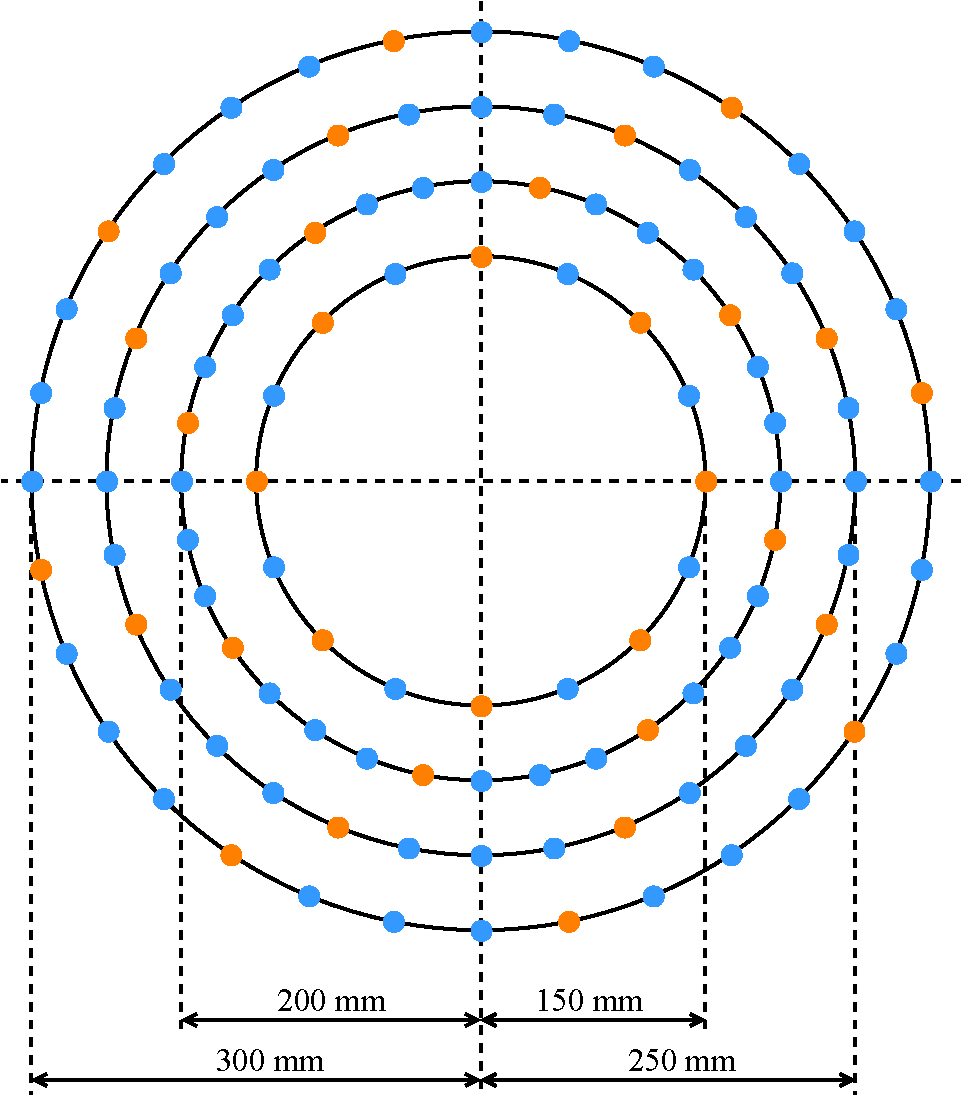
\includegraphics[width=7cm]{images/5_array_evaluation/prototype_array_multi_circular.pdf}
		\centering
		\caption{Multi-Circular Array}
		\label{fig:prototype_array_multi_circular}
	\end{wrapfigure}
	Lorem ipsum dolor sit amet, consetetur sadipscing elitr, sed diam nonumy eirmod tempor invidunt ut labore et dolore magna aliquyam erat, sed diam voluptua.
	At vero eos et accusam et justo duo dolores et ea rebum. Stet clita kasd gubergren, no sea takimata sanctus est Lorem ipsum dolor sit amet.
	Lorem ipsum dolor sit amet, consetetur sadipscing elitr, sed diam nonumy eirmod tempor invidunt ut labore et dolore magna aliquyam erat, sed diam voluptua.
	At vero eos et accusam et justo duo dolores et ea rebum.
	\todo[inline]{\@Alain: Add explanation of the array geometry here}
\end{minipage}
\vspace{0.5cm}    % Adjust this depending on the length of the text above

\subsection{Archimedean Spiral Array}
\begin{minipage}{\linewidth}
	\begin{wrapfigure}{r}{7.5cm}
		\vspace{-0.8cm}
		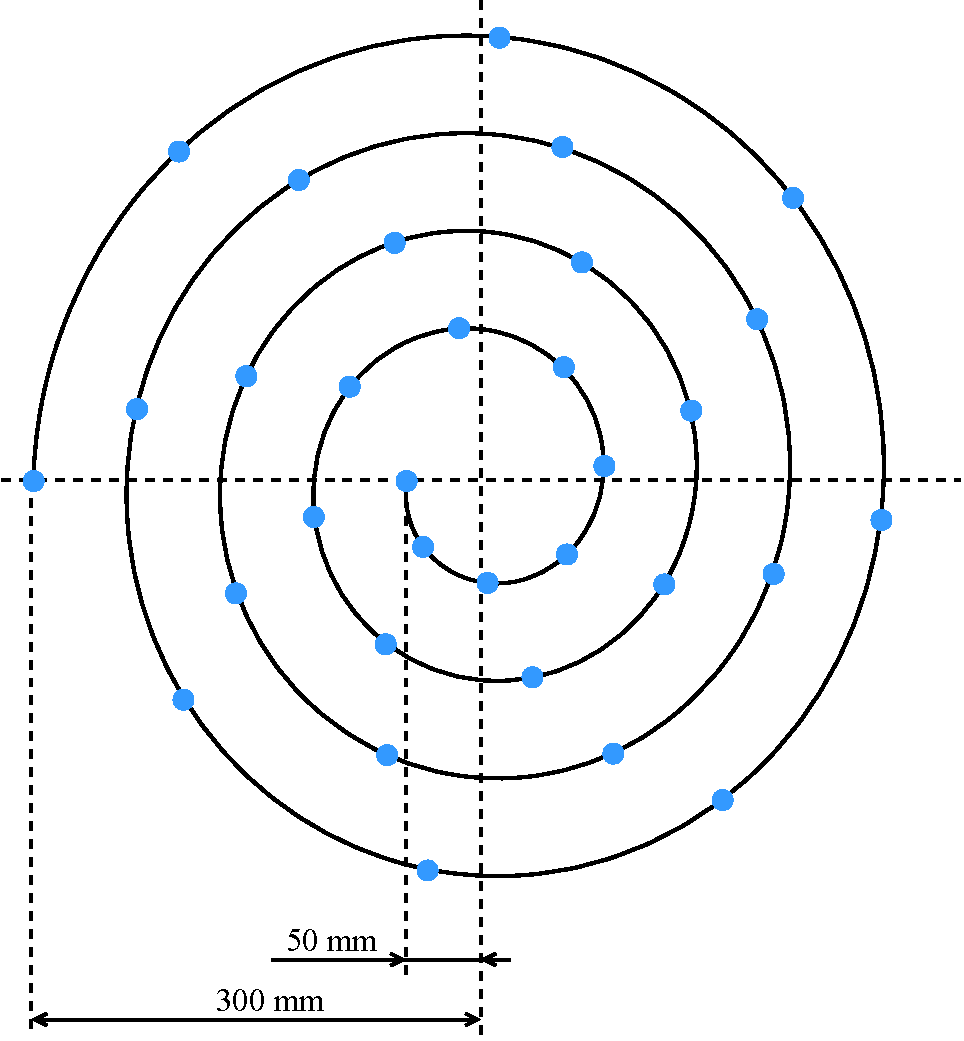
\includegraphics[width=7cm]{images/5_array_evaluation/prototype_array_archimedian_spiral.pdf}
		\centering
		\caption{Archimedean Spiral Array}
		\label{fig:prototype_array_archimedian_spiral}
	\end{wrapfigure}
	Lorem ipsum dolor sit amet, consetetur sadipscing elitr, sed diam nonumy eirmod tempor invidunt ut labore et dolore magna aliquyam erat, sed diam voluptua.
	At vero eos et accusam et justo duo dolores et ea rebum. Stet clita kasd gubergren, no sea takimata sanctus est Lorem ipsum dolor sit amet.
	Lorem ipsum dolor sit amet, consetetur sadipscing elitr, sed diam nonumy eirmod tempor invidunt ut labore et dolore magna aliquyam erat, sed diam voluptua.
	At vero eos et accusam et justo duo dolores et ea rebum.
	\todo[inline]{\@Alain: Add explanation of the array geometry here}
\end{minipage}
\newpage


\subsection{Wooden Prototype Arrays}
Two wooden prototypes, a multi-circular array and an Archimedean spiral array, were manufactured by laser-cutting 5\,mm plywood.
Both arrays had to be split into several pieces due to the limited size of the laser-cutter and were later glued together.
In the centre of each array, a mechanical mount for the Acquisition-System hardware was integrated.
\begin{figure}[h!]
	\centering
	\begin{minipage}{0.49\textwidth}
		\centering
		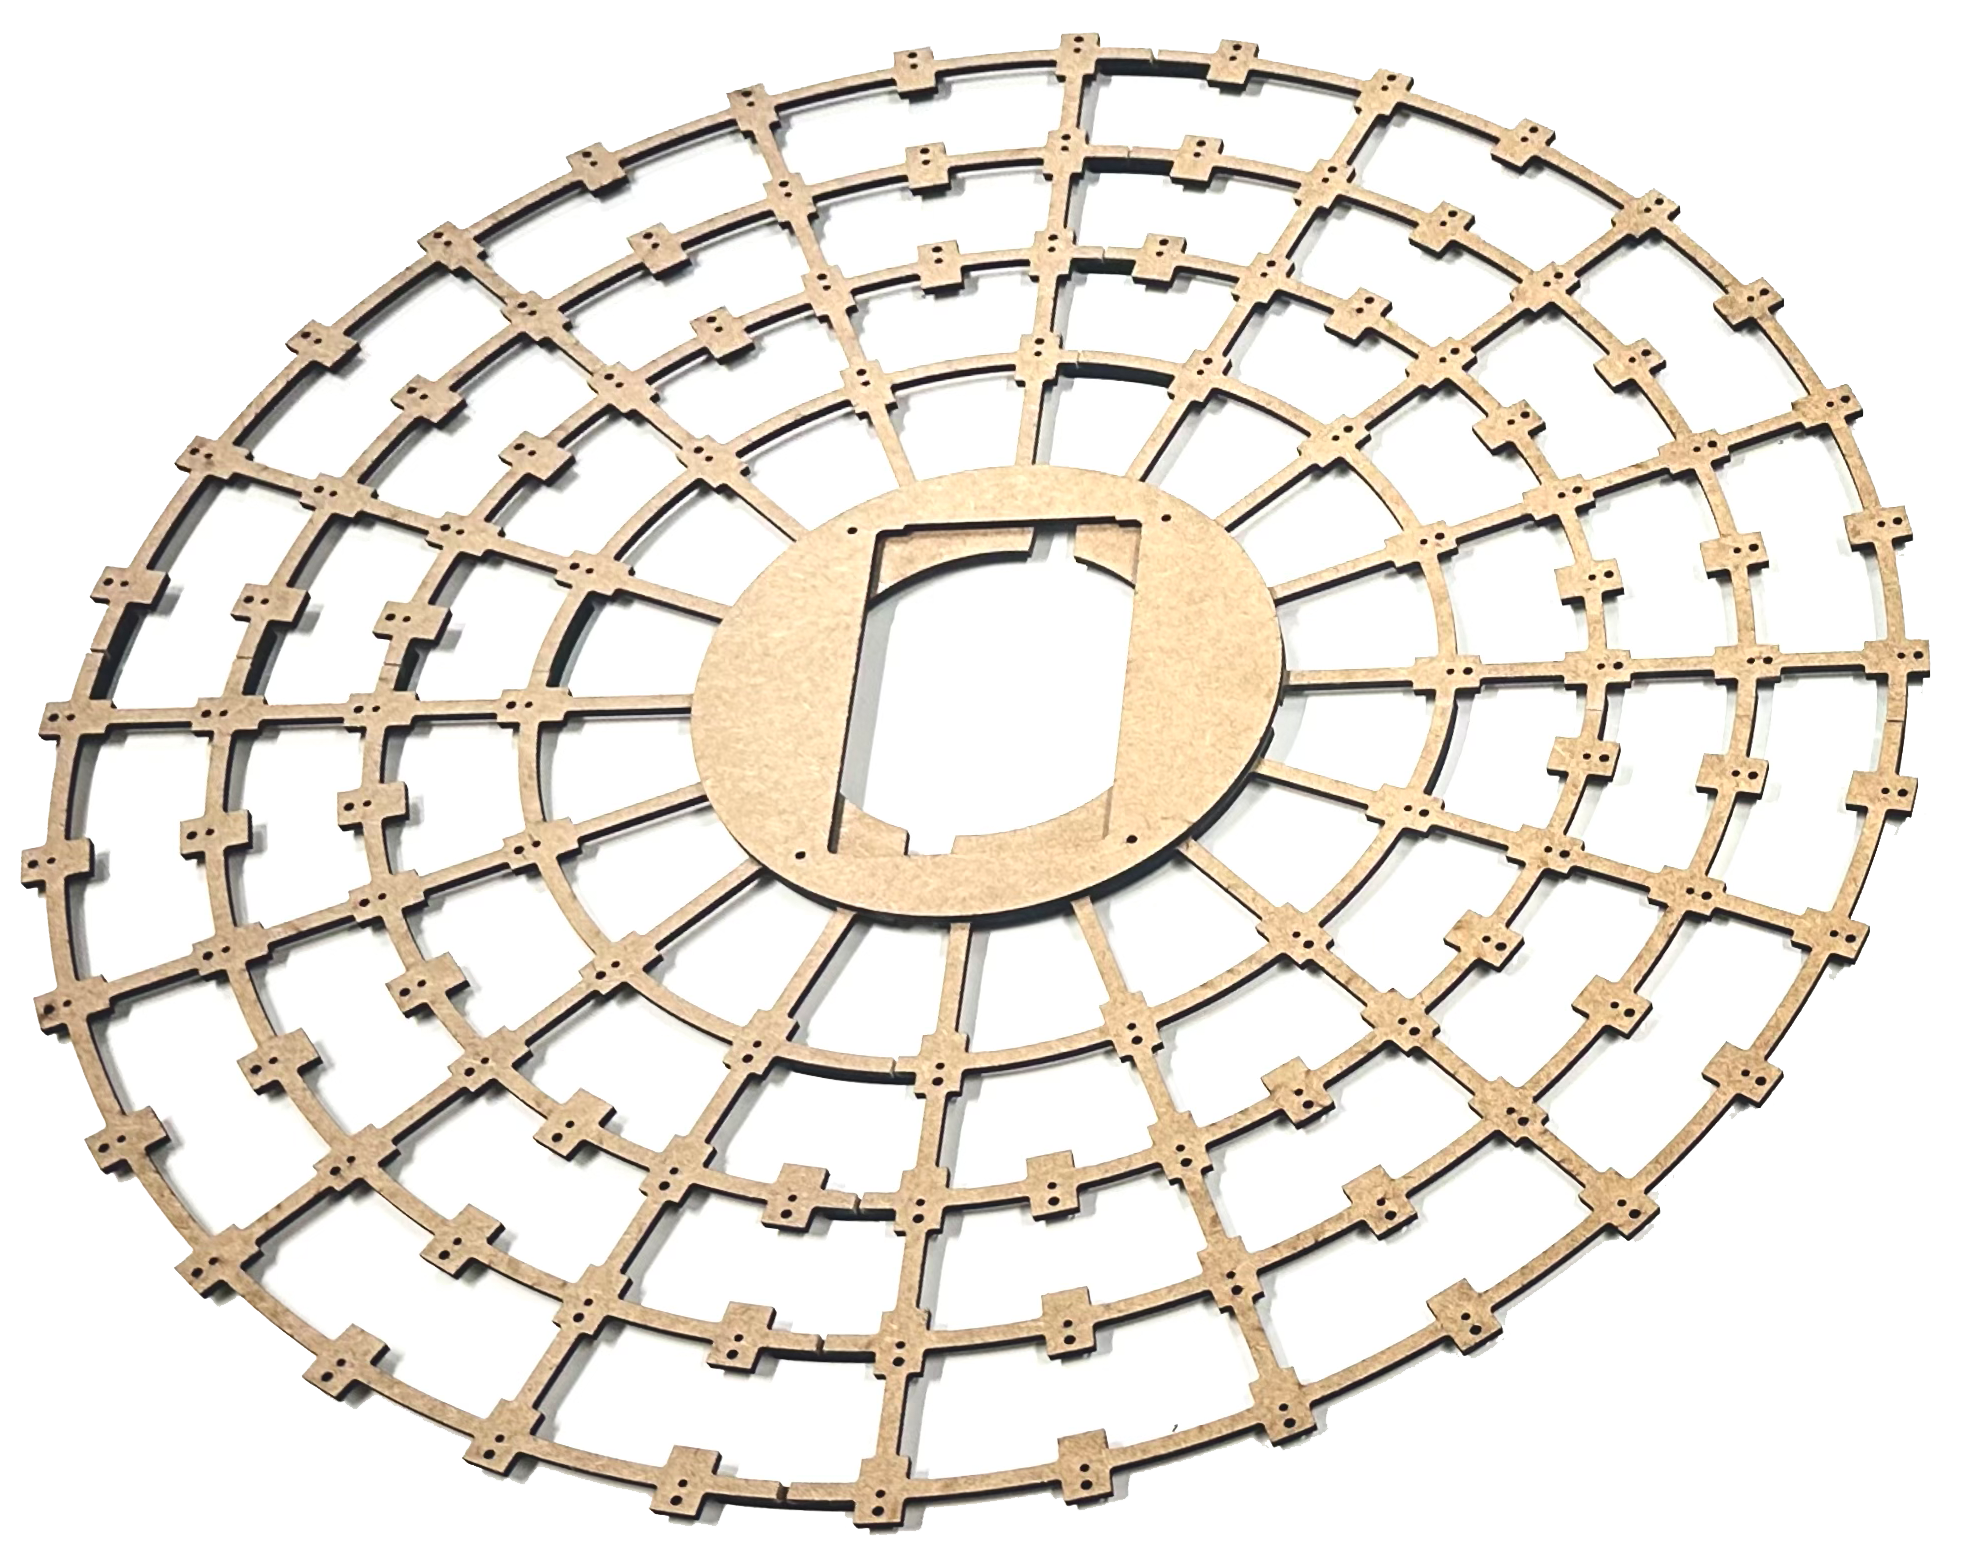
\includegraphics[width=0.95\textwidth]{images/5_array_evaluation/wooden_circular_array.png}
		\caption{Wooden Circular Array}
		\label{fig:wooden_circular_array}
	\end{minipage}
	\begin{minipage}{0.49\textwidth}
		\centering
		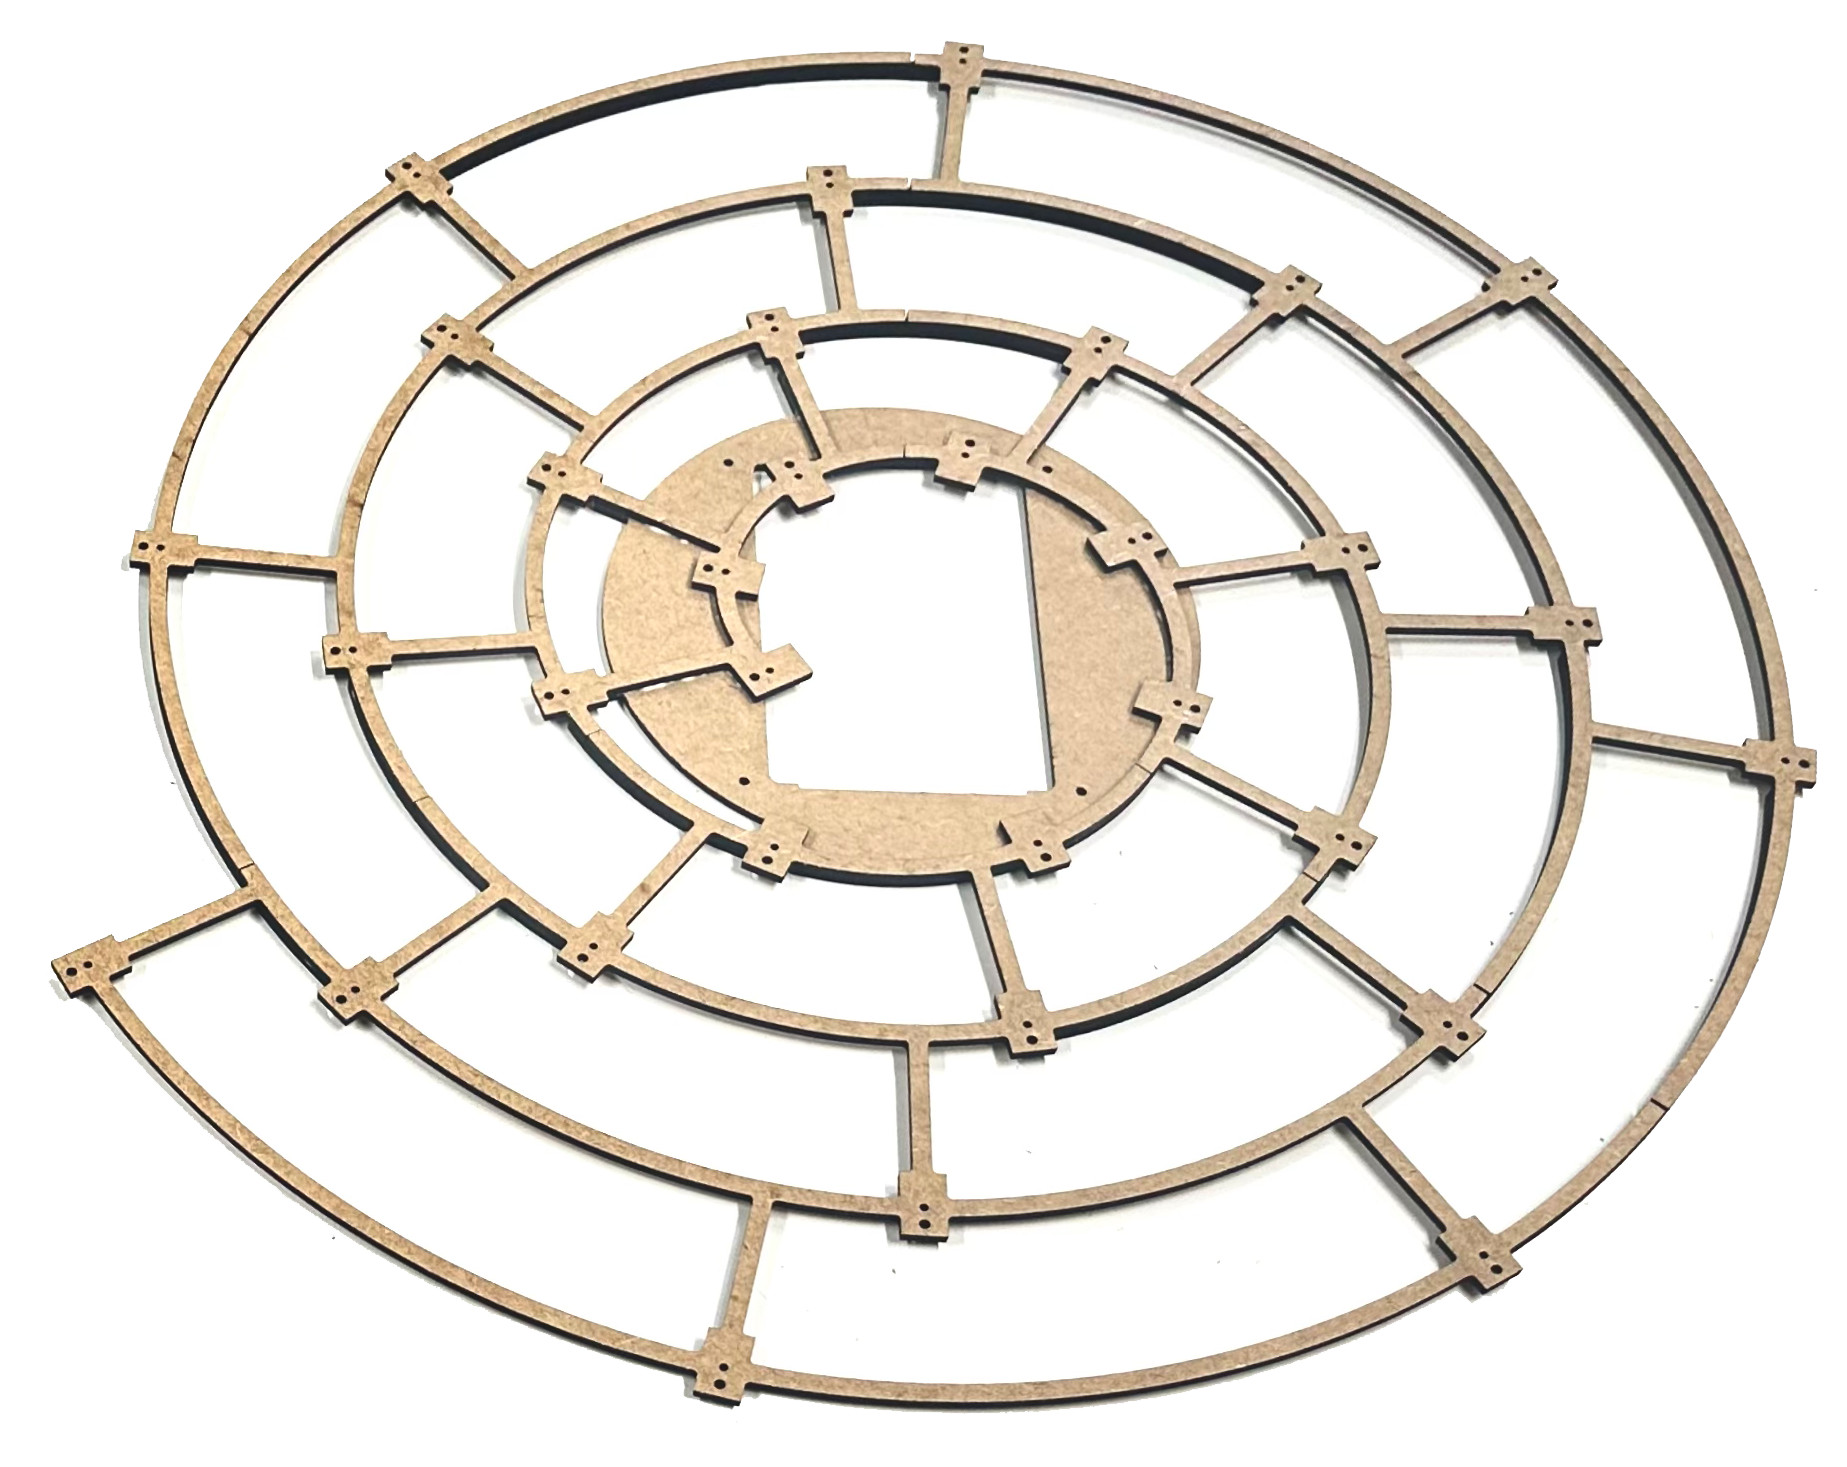
\includegraphics[width=0.95\textwidth]{images/5_array_evaluation/wooden_archimedean_spiral_array.png}
		\caption{Wooden Archimedean Spiral Array}
		\label{fig:wooden_archimedean_spiral_array}
	\end{minipage}
\end{figure}


\newpage
\section{Measurements \& Findings} \label{sec:array_prototype_measurements}
Blabla

\todo[inline]{Describe why we used fluffy stuff on the microphones (because we had problems first with wind). Mention the wind protection furr made by RØDE called DeadWombat.}


\begin{figure}[h!]
	\centering
	\begin{minipage}{0.49\textwidth}
		\centering
		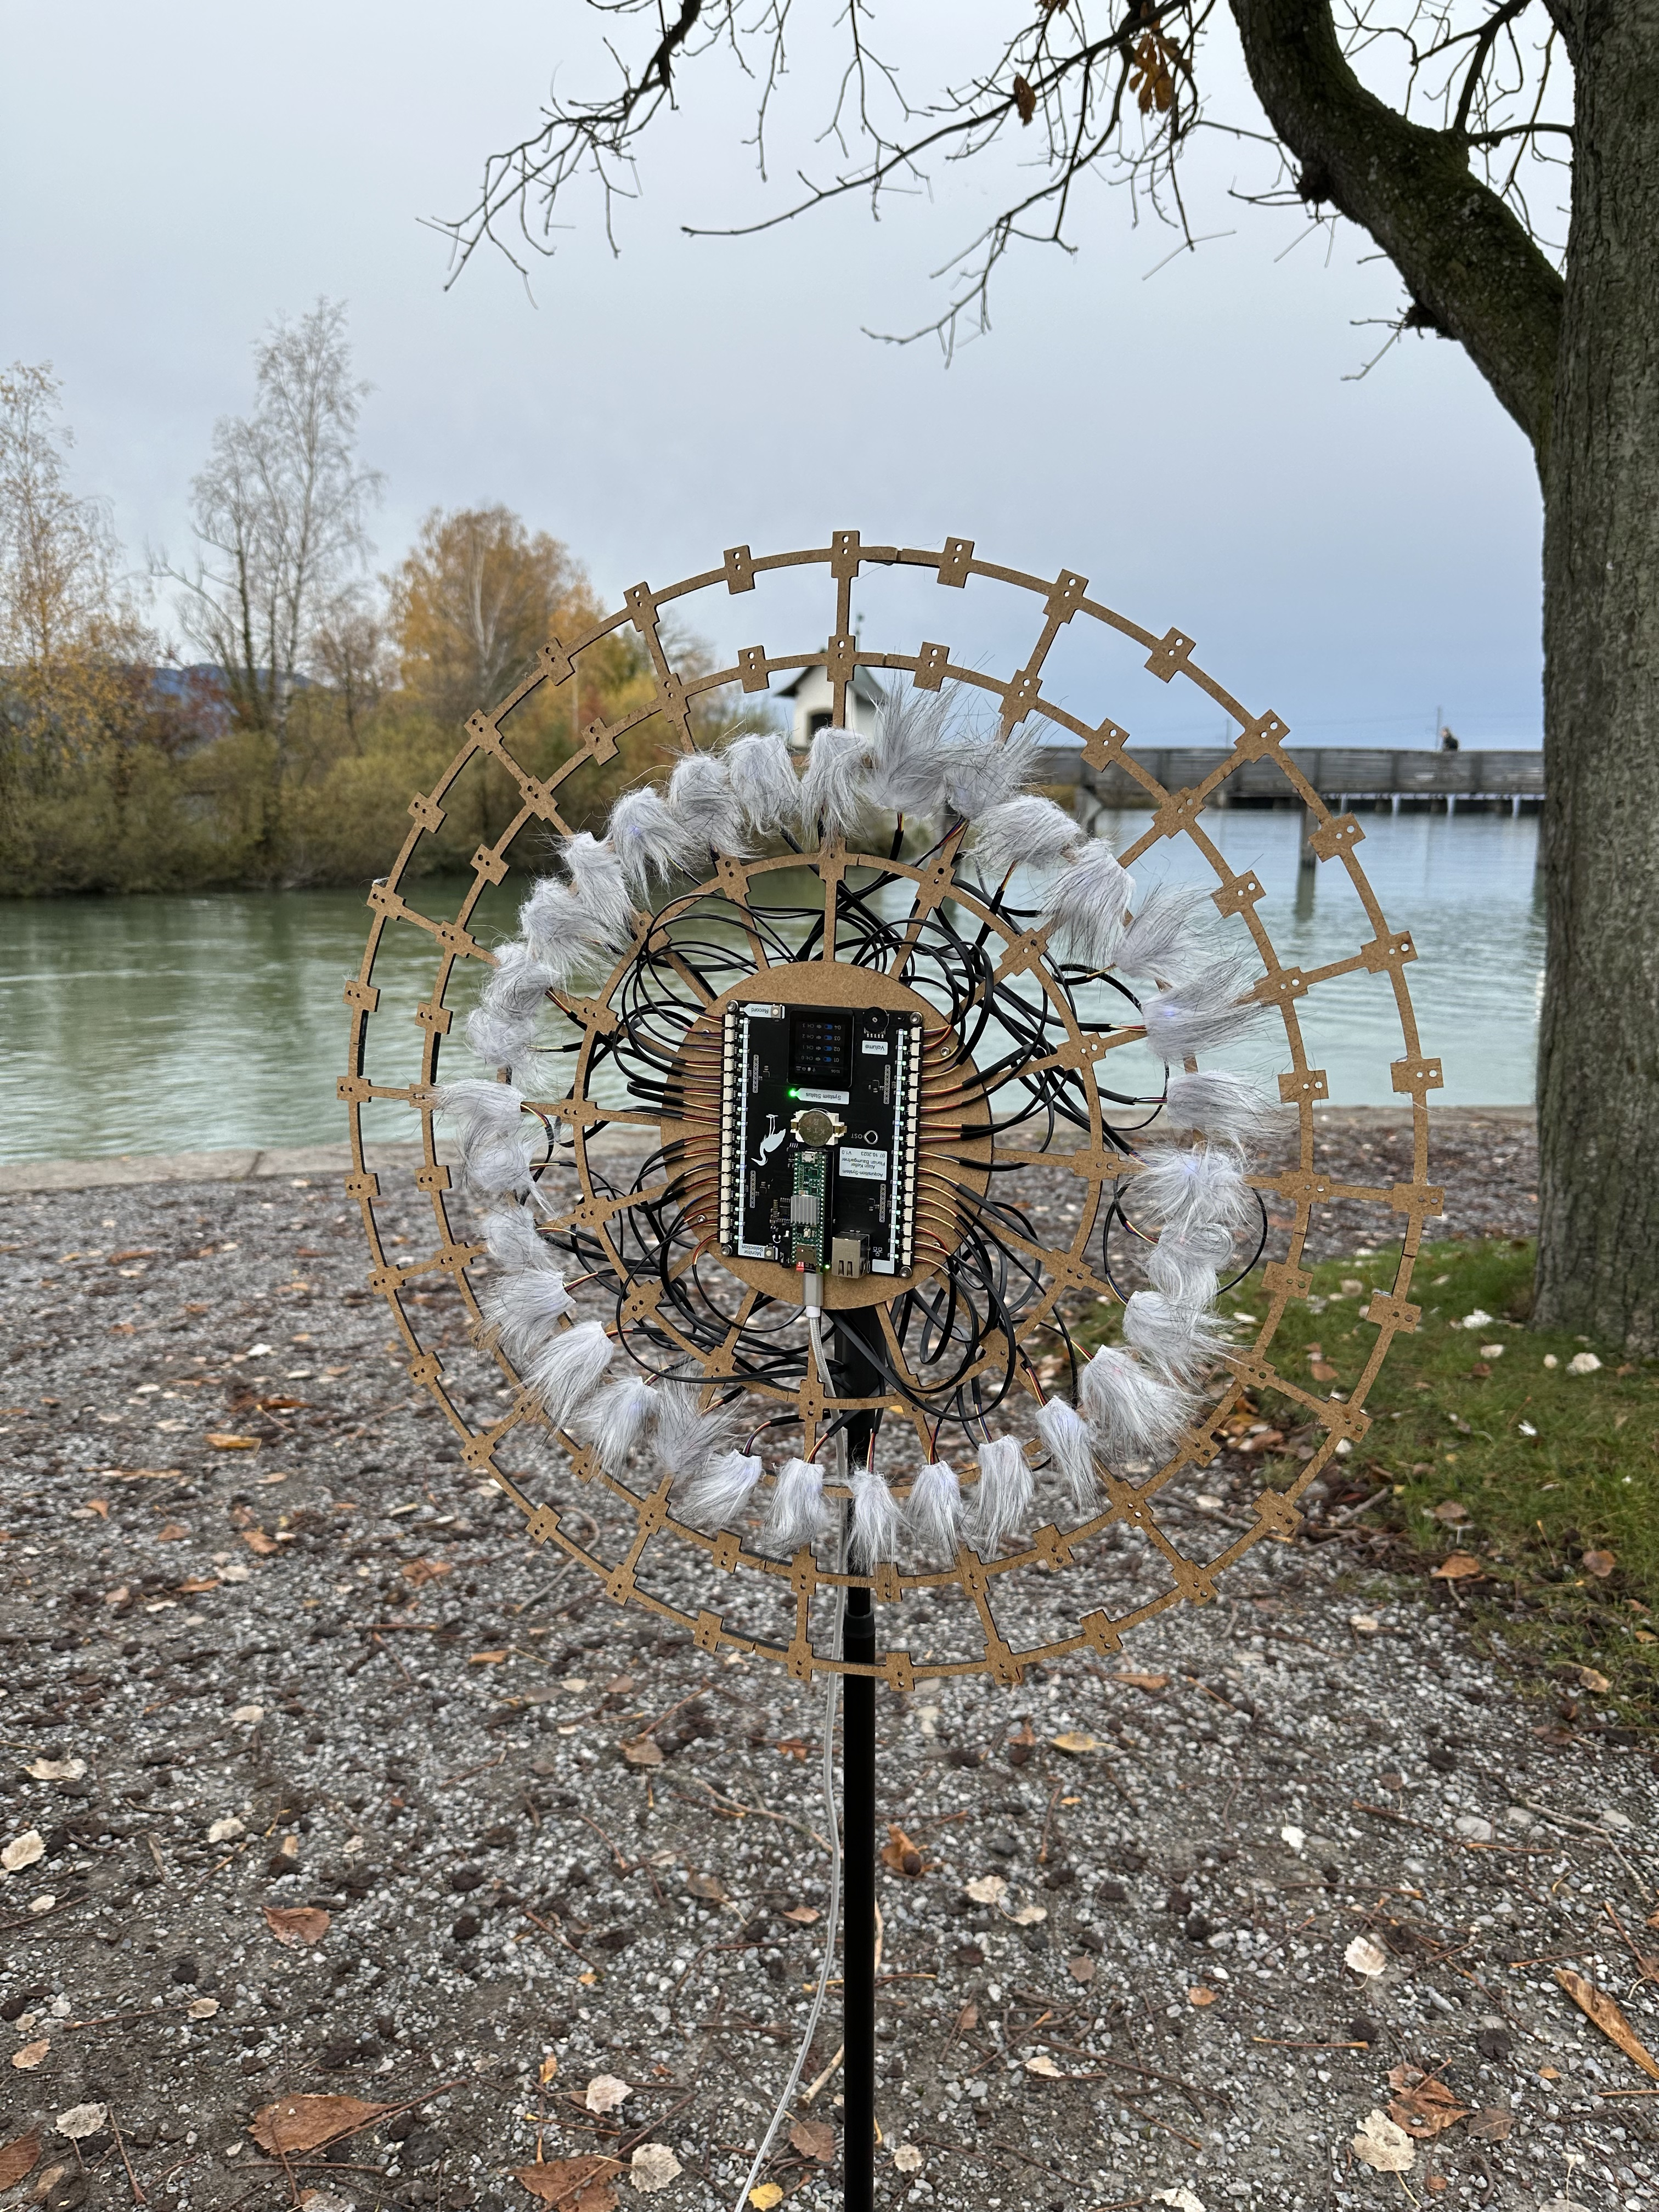
\includegraphics[width=0.95\textwidth]{images/5_array_evaluation/array_test_1.jpg}
		\caption{Multi-Circular Array (inner circle)}
		\label{fig:array_test_1}
	\end{minipage}
	\begin{minipage}{0.49\textwidth}
		\centering
		\includegraphics[width=0.95\textwidth]{images/5_array_evaluation/array_test_2.jpg}
		\caption{Multi-Circular Array (interleaved  pattern)}
		\label{fig:array_test_2}
	\end{minipage}
\end{figure}

\todo[inline]{Conclusion of array geometry → tree-dimensional array may provide better results. (This will be referenced in chapter of final design)}



\newpage
\section{Final Array Design}
Blabla

\begin{figure}[h]
	\centering
	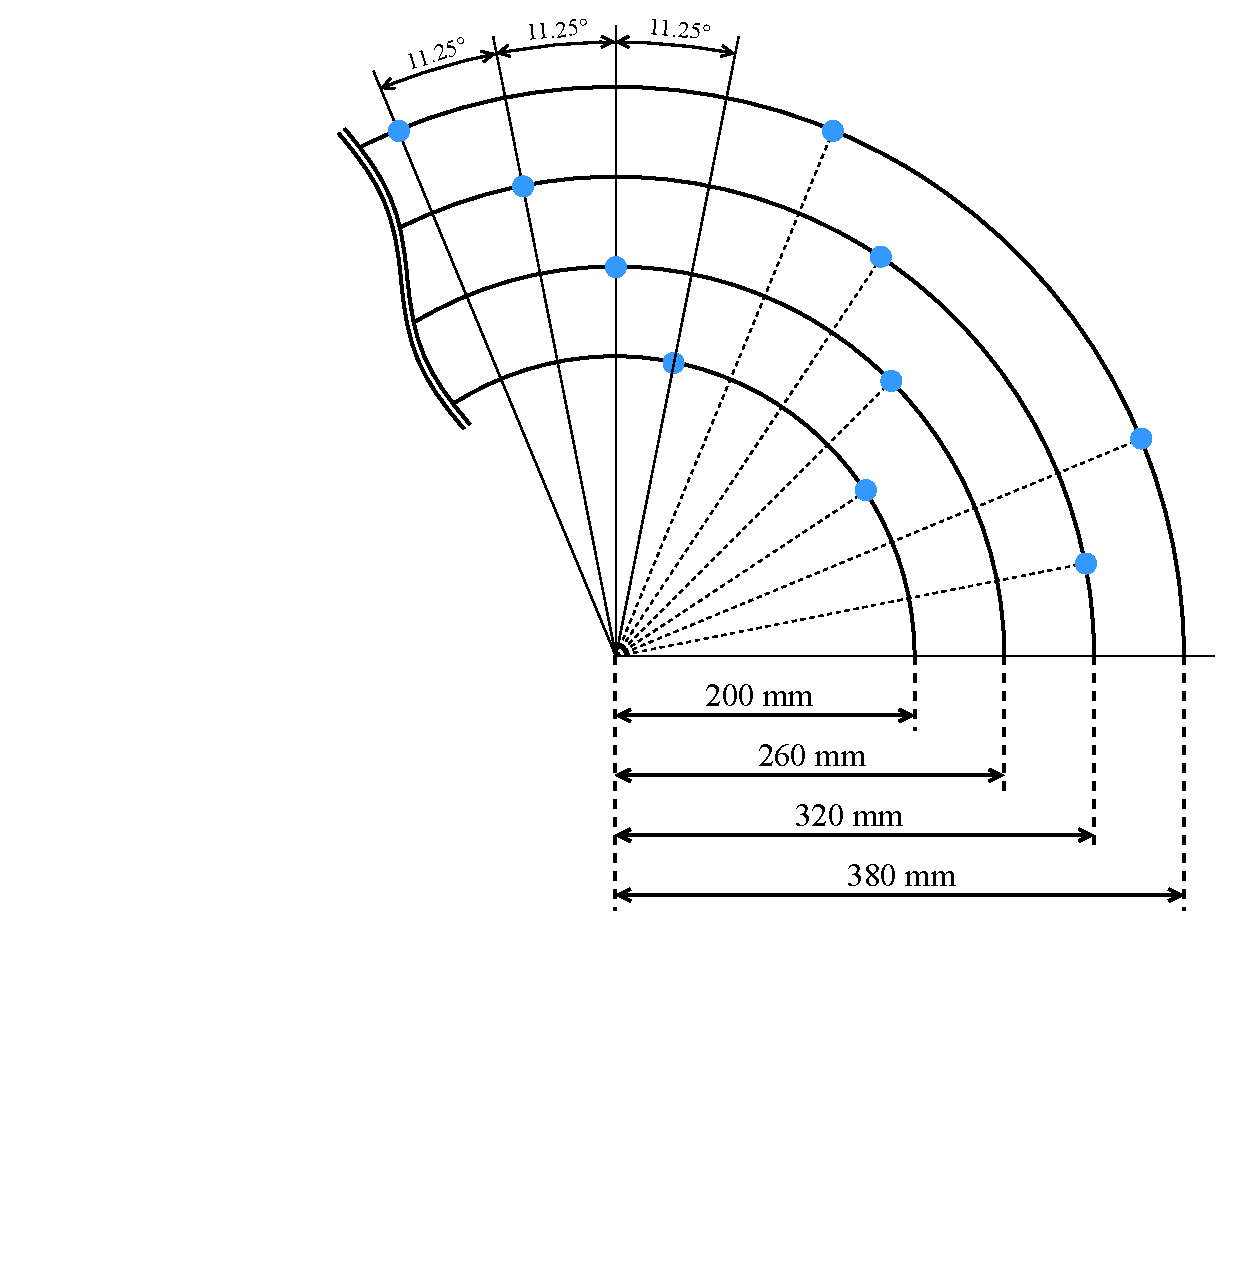
\includegraphics[width=0.75\textwidth, trim={5.5cm 6.0cm 0 0}]{images/5_array_evaluation/final_array_concept_design.pdf}
	\caption{Final Array Concept Design}
	\label{fig:final_array_concept_design}
\end{figure}
